\documentclass[aps,prb,
superscriptaddress,
,twocolumn
,floatfix,footinbib,longbibliography,
%preprint
]{revtex4-2}
%\documentclass[aps,preprint,floatfix,footinbib,longbibliography]{revtex4-1}
\usepackage{epsfig}
\usepackage{graphicx}% Include figure files
\usepackage{dcolumn}% Align table columns on decimal point
\usepackage{bm}% bold math
\usepackage{mathrsfs}
\usepackage{amsmath}
\usepackage{bbold}
\usepackage{color,xcolor}
\usepackage{epstopdf}
\usepackage{subfigure}
\usepackage{footmisc}
%\newcommand{\equt}[1]{\stackrel{#1}{=}}
%\usepackage[backend=bibtex,sorting=none,style=trad-abbrv,citestyle=numeric]{biblatex}

%\usepackage[sorting=none]{biblatex}
%\usepackage{hyperref}
%\usepackage[titletoc]{appendix}
% avoids incorrect hyphenation, added Nov/08 by SSR
\hyphenation{ALPGEN}
\hyphenation{EVTGEN}
\hyphenation{PYTHIA}

\usepackage[colorlinks=true,pdfborder=001,linkcolor=blue,anchorcolor=blue,citecolor=blue,urlcolor=blue]{hyperref}

\newcommand{\revision}[1]{{\color{blue}{#1}}}
\newcommand{\JT}[1]{{\color{red}{#1}}}
\begin{document}


%\title{Controlling photon statistics by Fano-like interference effect in a cavity with two molecules}

\title{Effective control of photon statistics from electroluminescence by Fano-like interference effect}

\author{Lei-Lei Nian}
\affiliation{School of Physics and Wuhan National High Magnetic Field Center, Huazhong University of Science and Technology, Wuhan 430074, P. R. China}
\author{Tao Wang}
\affiliation{School of Physics and Wuhan National High Magnetic Field Center, Huazhong University of Science and Technology, Wuhan 430074, P. R. China}
\author{Zu-Quan Zhang}
\affiliation{Department of Physics, National University of Singapore, Singapore 117551, Republic of Singapore}
\author{Jian-Sheng Wang}
%\email{phywjs@nus.edu.sg}
\affiliation{Department of Physics, National University of Singapore, Singapore 117551, Republic of Singapore}
\author{Jing-Tao L\"{u}}
\email{jtlu@hust.edu.cn}
\affiliation{School of Physics and Wuhan National High Magnetic Field Center, Huazhong University of Science and Technology, Wuhan 430074, P. R. China}




\date{\today}% It is always \today, today,
             %  but any date may be explicitly specified
\begin{abstract}
Photon blockade induced by optical nonlinearity has been widely used to generate single-photon emission under optical driving in quantum optics. However, the same approach is difficult to achieve in electrically driven molecular junctions. Here we propose a scheme for tuning photon statistics via Fano-like interference effect in a system consisting of two molecules within one optical cavity.
Under electrical pumping, a transition from photon bunching to anti-bunching takes place as a manifestation of the Fano-like interference. This effect persists even in presence of the dipole-dipole interaction between molecules based on the parameters extracted from experiments.
Our proposal can be realized in current-carrying scanning tunneling microscope junctions.


%\begin{description}
%\item[PACS numbers]
%73.63.Kv, 73.23.-b, 71.38.-k, 72.25.-b
%\end{description}
\end{abstract}

%\pacs{73.63.kv, 73.23.-b, 71.38.-k}% PACS, the Physics and Astronomy
                             % Classification Scheme.
%\keywords{Suggested keywords}%Use showkeys class option if keyword
                              %display desired
\maketitle

\section{Introduction}
The investigation of single-photon sources has recently attracted considerable
interest because of its potential applications in quantum computation and quantum communication \cite{knill2001scheme,walther2005experimental,ladd2010quantum,RevModPhys.81.1301}.
Creating single photon as well as exploiting its various applications constitute the principle
tasks of quantum optics, quantum chemistry, and condensed matter physics. In quantum optics, single-photon
emission can be obtained with the help of photon blockade, which is caused by the strong optical nonlinearity of the considered systems
\cite{blinov2004observation,dayan2008photon,faraon2008coherent,PhysRevLett.107.063601,PhysRevLett.106.243601,PhysRevLett.118.133604}.
On the other hand, the destructive quantum
interference between different excitation pathways can also be used to generate single-photon
emission \cite{PhysRevLett.104.183601,PhysRevLett.108.183601,PhysRevA.88.033836,PhysRevA.90.043822,PhysRevA.98.053801}. It does not need strong optical nonlinearity of the system, so it is usually called the unconventional photon blockade. 
%Moreover, the strong photon anti-bunching can also be induced by quantum interference effects driven by coherent pumping\cite{PhysRevLett.105.263601,PhysRevLett.122.173603,PhysRevLett.108.183601}.

In quantum chemistry and condensed matter physics, means of generating single photon are different from that of photon blockade in quantum optics
\cite{yuan2002electrically,merino2015exciton,roslawska2018single,roslawska2020atomic}. One of the most effective ways to generate single-photon emission is through controlled radiation of single emitters, such as single atom \cite{PhysRevLett.39.691}, quantum dot \cite{yuan2002electrically}, color center \cite{mizuochi2012electrically}, or single molecule \cite{nothaft2012electrically}. To date, single molecule emitter has become one of the desired candidates due to its high stability and controllable light emission \cite{qiu2003vibrationally,wu2006atomic,dong2010generation, PhysRevLett.109.186601,jiang2015distinguishing,zhang2016visualizing,PhysRevLett.122.233901,wu2019controllable,PhysRevLett.122.177401,dong2020microscopic,doppagne2020single}.
%
Recently, single-photon emission has been observed experimentally in single molecule or molecular chains decoupled from metal substrate driven
by the inelastic tunneling electrons injected from a scanning tunneling microscope (STM) tip \cite{zhang2017electrically,PhysRevLett.122.233901}. Considering a simple model that contains a single-level molecule interacting with a single plasmon mode, single-electron tunneling allows to achieve single-photon emission \cite{PhysRevLett.123.246601}. However, it takes place only in the strong molecule-plasmon coupling regime.
Actually, in molecule-mediated STM junctions, the coherent coupling between molecular exciton and plasmon cavity provides an effective way to tune the emission spectrum,
resulting in Fano line shape observed experimentally \cite{PhysRevLett.116.036802,zhang2017sub,PhysRevLett.119.013901}
and explained theoretically \cite{nian2018fano,nian2019mechanism}.
But, so far, how this coupling affects photon statistics has not been revealed.


In this paper, we fill this gap by analyzing a model system consisting of two molecules within one optical cavity.
The schematic setup is illustrated in Fig.~\ref{junction-1}. The molecule $p$ ($m$) can be excited by electrical pumping $E_{p}$ ($E_{m}$). The excited molecules are coupled to an optical cavity characterized by parameters $g_{p}$ and $g_{m}$. The dipole-dipole interaction between molecules is considered and characterized by parameter $t_{D}$. Meanwhile, the system is assumed to interact weakly with the environment. 
We consider strong Coulomb interaction in each molecule, such that the corresponding molecule can only be occupied by one electron. In experiment, our model can be realized by injecting an electron and a hole into the levels $e/l$ and $g/h$ from electrodes, respectively. 


Using the quantum master equation, we can study the statistical properties of photons in the cavity.
The photons emitted from single- and two-molecule setup (see Fig.~\ref{junction-1} for explanation of different setups) exhibit a bunching behavior, while a strong photon anti-bunching can be achieved in a system with Fano-like interference \footnote{Fano interference is caused by the interference between a discrete state and a continuous state. Here, the excitation of the molecule $m$ and the cavity mode act as the discrete state and continuous state, respectively. However, for the cavity with low-dissipation, both channels are discrete states, so we name this effect as Fano-like interference effect.}.
In fact, the system with single molecule coupled to the cavity can emit antibunched photons in the bad-cavity regime \cite{PhysRevB.70.115304,PhysRevA.91.061804,zhang2017electrically,PhysRevLett.122.233901}.
However, our results show that the single-photon statistics can be further enhanced by the Fano-like effect.
More importantly, photons in coherent and bunched states can be tuned to strong anti-bunched state by the Fano-like effect in the good-cavity regime. We further show that the anti-bunched state is stable against inter-molecule dipole-dipole interaction with parameters extracted from experiments.

\revision{The mechanism of using Fano-like interference driven by electrical pumping for single photon emission has two advantages. First, the interference can be achieved by positioning a molecule nearby a molecule-mediated cavity. 
 Meanwhile, single-photon emission from single molecule in current-carrying molecular junctions has already been realized experimentally \cite{PhysRevLett.116.036802,zhang2017sub,PhysRevLett.119.013901,roslawska2020atomic},
and hence our prediction is within the experimental reach.
Second, contrary to previous proposal \cite{PhysRevLett.108.183601} where single photon emission is only possible in the bad-cavity limit, our proposal may be realized in a much broader range of the cavity quantity factor.}

\begin{figure}
\centering
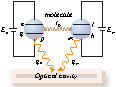
\includegraphics[width=0.3\textwidth]{junction-1.pdf}
\caption{Schematic representation of the system: two molecules (marked by $p$ and $m$) and an optical cavity. The molecules can be excited by electrical pumping ($E_{p}$ and $E_{m}$) and they couple to the cavity by their respective electron-photon interactions characterized by parameters $g_{p}$ and $g_{m}$. The dipole-dipole interaction between molecules is characterized by $t_{D}$. The dissipation of the molecules and the cavity are included in the theory but not shown here. Here we consider three situations: (1) Single-molecule emission, where $E_{m}=0$ and $g_{m}=0$. This corresponds to the Jaynes-Cummings model. (2) Emission with Fano-like interference, where $E_{m}=0$ and $g_{m}\neq 0$; (3) Two-molecule emission, where $E_{m}\neq 0$ and $g_{m}\neq 0$. This corresponds to the Tavis-Cummings model. In all cases, the molecule $p$ is always excited by an electrical pumping and its coupling with cavity is considered, that is, $E_{p}\neq 0$ and $g_{p}\neq 0$. }
\label{junction-1}
\end{figure}

\section{Model}
A schematic of the model is shown in Fig.~\ref{junction-1}.
The two molecules labeled by $p$ and $m$ can be excited by the electrical pumping $E_{p}$ and $E_{m}$, respectively.
They couple simultaneously to one optical cavity.
The total Hamiltonian is
\begin{equation}
\mathcal{H}_{s}=\mathcal{H}_{p}+\mathcal{H}_{m}+\mathcal{H}_{c}+\mathcal{H}_{I}+\mathcal{H}_{D},
\label{Hamiltonian}
\end{equation}
where $\mathcal{H}_{p}$ and $\mathcal{H}_{m}$ describe the uncoupled molecules
\begin{equation}
\begin{split}
&\mathcal{H}_{p}=\sum_{i=g,e}\varepsilon_{i}d_i^\dagger d_i,\\
&\mathcal{H}_{m}=\sum_{i^{\prime}=h,l}\varepsilon_{i^{\prime}}d_{i'}^\dagger d_{i'},\\
\end{split}
\end{equation}
where each molecule contains two well-defined energy levels, that is, $g/e~(h/l)$ for $p~(m)$ with energies $\varepsilon_{g/e}~(\varepsilon_{l/h})$.
The optical cavity mode is considered as  a single harmonic oscillator with angular frequency $\omega_{c}$
\begin{equation}
\mathcal{H}_{c}=\left(\frac{1}{2}+\hbar\omega_{c}\right)a^{\dag}_{c}a_{c}.
\end{equation}
The interaction between the two molecules and the cavity in the rotating wave approximation is
\begin{equation}
\mathcal{H}_{I}=g_{p}(\sigma_{p}a^{\dag}_{c}+a_{c}\sigma_{p}^{\dag})+g_{m}(\sigma_{m}a^{\dag}_{c}+a_{c}\sigma_{m}^{\dag}),
\end{equation}
where $\sigma_{p}=d_g^\dagger d_e$ ($\sigma_{m}=d_h^\dagger d_l$) and $\sigma_{p}^{\dag}=d_e^\dagger d_g$ ($\sigma_{m}^{\dag}=d_l^\dagger d_h$) are the annihilation and creation operators of molecular exciton $p$ ($m$), respectively, and $g_{m}$, $g_{p}$ are the corresponding molecule-cavity coupling strength.
We will also consider a dipole-dipole coupling between the two molecules
\begin{equation}
\mathcal{H}_{D}=t_{D}(\sigma_{p}^{\dagger}\sigma_{m}+\sigma_{m}^{\dagger}\sigma_{p}),
\end{equation}
where $t_{D}$ is the coupling strength \cite{vlaming2014tunable,zhang2016visualizing,PhysRevLett.122.233901}.

%\revision{The Hamiltonian of the environment and its interaction with the system is provided in Section I of the Supplemental Material \cite{SupplementalMaterial}.}




\section{Master equation}
Considering weak interaction between the system and the environment (details are given in the Supplemental Materials \cite{SupplementalMaterial}), we can use the master equation to describe photon transport and its statistics.
We define the reduced density matrix for the system as $\rho$ by tracing out the environment degrees of freedom in the total density matrix $\rho_{t}$, that is, $\rho={\rm Tr}_{\rm en}[\rho_{t}]$. Under the Born-Markovian approximation, the dynamics of $\rho$ satisfies the master equation \cite{gardiner1985handbook,scully1997quantum,breuer2002theory,carmichael2013statistical}
\begin{equation}
\begin{split}
\frac{d}{dt}\rho&=\frac{1}{i\hbar}[\mathcal{H}_{s},\rho]\\
&+\frac{1}{2}\sum_{\nu=p,m}\Gamma^{+}_{\nu}\mathcal{L}[\sigma_{\nu}^{\dagger}]\rho
+\frac{1}{2}\sum_{\nu=p,m}\Gamma^{-}_{\nu}\mathcal{L}[\sigma_{\nu}]\rho\\
&+\frac{1}{2}\sum_{\nu=p,m}\gamma^{+}_{d\nu}\mathcal{L}[\sigma_{\nu}^{\dagger}]\rho
+\frac{1}{2}\sum_{\nu=p,m}\gamma^{-}_{d\nu}\mathcal{L}[\sigma_{\nu}]\rho\\
&+\frac{1}{2}\kappa^{+}_{c}\mathcal{L}[a_{c}^{\dagger}]\rho
+\frac{1}{2}\kappa^{-}_{c}\mathcal{L}[a_{c}]\rho.
\end{split}
\label{master-equation}
\end{equation}
Here, the commutator in the first \revision{line} at the right hand side describes the coherent evolution of the isolated $\mathcal{H}_{s}$.
The system coupling with the environment is taken into account by the rest terms. %\cite{PhysRevA.59.4756,PhysRevB.79.235325,PhysRevB.79.235326}.
\revision{The electrical driving applied to the molecule p (m) is described by the two terms in the second line. %an electron-hole pair can be injected from the corresponding electrodes $\nu$ with the help of voltage bias.
%Note that, the electronic reservoir is not in thermodynamic equilibrium.
%where the energy comes from electron-hole recombination, 
%i.e., inelastic electronic transition from high to low energy states. 
%The reverse process characterized by the third term describes the creation of an electron-hole pair in the electrical reservoir. 
The two processes represented by $\Gamma^{+}_{\nu}$ and $\Gamma^{-}_{\nu}$ correspond to creation and recombination of molecular exciton, respectively.
A microscopic model of the electrical driving is given in Ref.~\cite{SupplementalMaterial}.}
%The driving rates for these two processes are  $\Gamma^{+}_{\nu}=E_{\nu}f^{e}_{j}$ and $\Gamma^{-}_{\nu}=E_{\nu}(1-f^{e}_{j})$, respectively.
%Here $f_{j}^{e}$ is the distribution function of the electronic reservoir.} 
%In fact, the electrodes under the applied bias can be regarded as a bosonic bath, then $E^{+/-}_{p/m}$ can be obtained by using the Fermi's golden rule \cite{PhysRevLett.107.046801,hu2020nonequilibrium}
%\begin{equation}
%\begin{split}
%E^{+/-}_{p}&=-\frac{2\pi}{\hbar}\sum_{i\in\alpha,f\in\beta}|\langle f\beta|M|i\alpha\rangle|^{2}[f_{\alpha/\beta}(\varepsilon_{i/j})-f_{\beta/\alpha}(\varepsilon_{f/i})]\\
%&\times n_{B}^{+/-}(\hbar\omega_{p}-eV)\delta(\varepsilon_{i}-\varepsilon_{f}\pm\varepsilon_{p}),
%\end{split}
%\end{equation}
%where $\omega_{p}=(\varepsilon_{e}-\varepsilon_{g})/\hbar$. $\varepsilon_{i}$ and $\varepsilon_{f}$ are the energies of electrons in electrodes with chemical potentials $\mu_{\alpha}$ and $\mu_{\beta}$, the applied bias between them is $eV=\mu_{\alpha/\beta}-\mu_{\beta/\alpha}>0$ for `$+/-$'. Moreover, $n_{B}^{+}=n_{B}$ and $n_{B}^{-}=n_{B}+1$.
%$M$ is the electron-photon coupling. One can get the expressions for $E^{+}_{m}$ and $E^{-}_{m}$ by replacing $\varepsilon_{p}$ with $\varepsilon_{m}$, where $\omega_{m}=(\varepsilon_{l}-\varepsilon_{h})/\hbar$.
%
The third and fourth lines describe the coupling of the molecular exciton and the cavity photon to the photon bath.
Specifically, $\gamma_{d\nu}^{-}=\gamma_{d\nu}[n_{B}(\omega_{\nu})+1]$ describes photon emission to the bath as a result of molecular exciton annihilation,  $\gamma_{d\nu}^{+}=\gamma_{d\nu}n_{B}(\omega_{\nu})$ corresponds to the opposite process of thermal excitation of the molecular exciton, which occurs only when the temperature of the bath is large enough. Here, $n_{B}(\omega)=(e^{\hbar\omega/k_{B}T}-1)^{-1}$ is the Bose-Einstein distribution.  The coupling between the cavity mode and the photon bath is written similarly with \revision{parameters $\kappa_c^{-}=\gamma_{c}[n_{B}(\omega_{c})+1]$ and $\kappa_c^{+}=\gamma_{c}n_{B}(\omega_{c})$}.
%
%
%and $f_{\alpha}(\varepsilon)=(e^{(\varepsilon-\mu_{\alpha})/k_{B}T}+1)^{-1}$ is the  Fermi-Dirac distribution.
The Lindblad superoperators act according to $\mathcal{L}[\mathcal{A}]\rho=2\mathcal{A}\rho \mathcal{A}^{\dagger}-\mathcal{A}^{\dagger}\mathcal{A}\rho-\rho\mathcal{A}^{\dagger}\mathcal{A}$, where $\mathcal{A}=\sigma_{\nu},\sigma_{\nu}^{\dagger},a_{p},a_{p}^{\dagger}$.
Here, we consider $T\approx0$ , such that $\Gamma^{-}_{\nu}\approx 0$, $\gamma_{d\nu}^{+}\approx0$, and $\kappa_{p}^{+}\approx0$. In this case, the molecular exciton can only be generated by electrical driving. It can further decay into the photon bath or to the cavity mode. 


To study the photon statistics in the cavity, we can calculate its equal-time $k$-th order coherence function $g^{(k)}(0)$ in the steady state
\begin{equation}
\begin{split}
g^{(k)}(0)=\dfrac{\langle a_{p}^{\dagger k} a_{p}^{k} \rangle}{\langle a_{p}^{\dagger} a_{p} \rangle^{k}}=\frac{\sum_{m}\prod_{l=0}^{k-1}(m-l)p_{m}}{(\sum_{m}mp_{m})^{k}},
\end{split}
\label{gn}
\end{equation}
where $p_{m}$ is the occupation probability of the cavity mode at state $|m\rangle$ (see Section II of Ref.~\cite{SupplementalMaterial} for details). 
The photon bunching and anti-bunching correspond to $g^{(2)}(0)>1$ and $g^{(2)}(0)<1$, respectively.


\section{Results}
In the following, we consider the photon emission from three different scenarios: (1) single-molecule emission; (2) emission with Fano-like interference; (3) two-molecule emission. The details of each setup are given in the caption of Fig.~\ref{junction-1}. In Figs.~\ref{fano-compare}-\ref{fano-rp}, we assume that the dipole-dipole interaction is zero, such that the effect of the Fano-like interference on photon statistics can be shown more clearly. In Fig.~\ref{fano-td}, we release this assumption and study the effect of dipole-dipole interaction on photon statistics. 
%
\begin{figure}[h]
\centering
%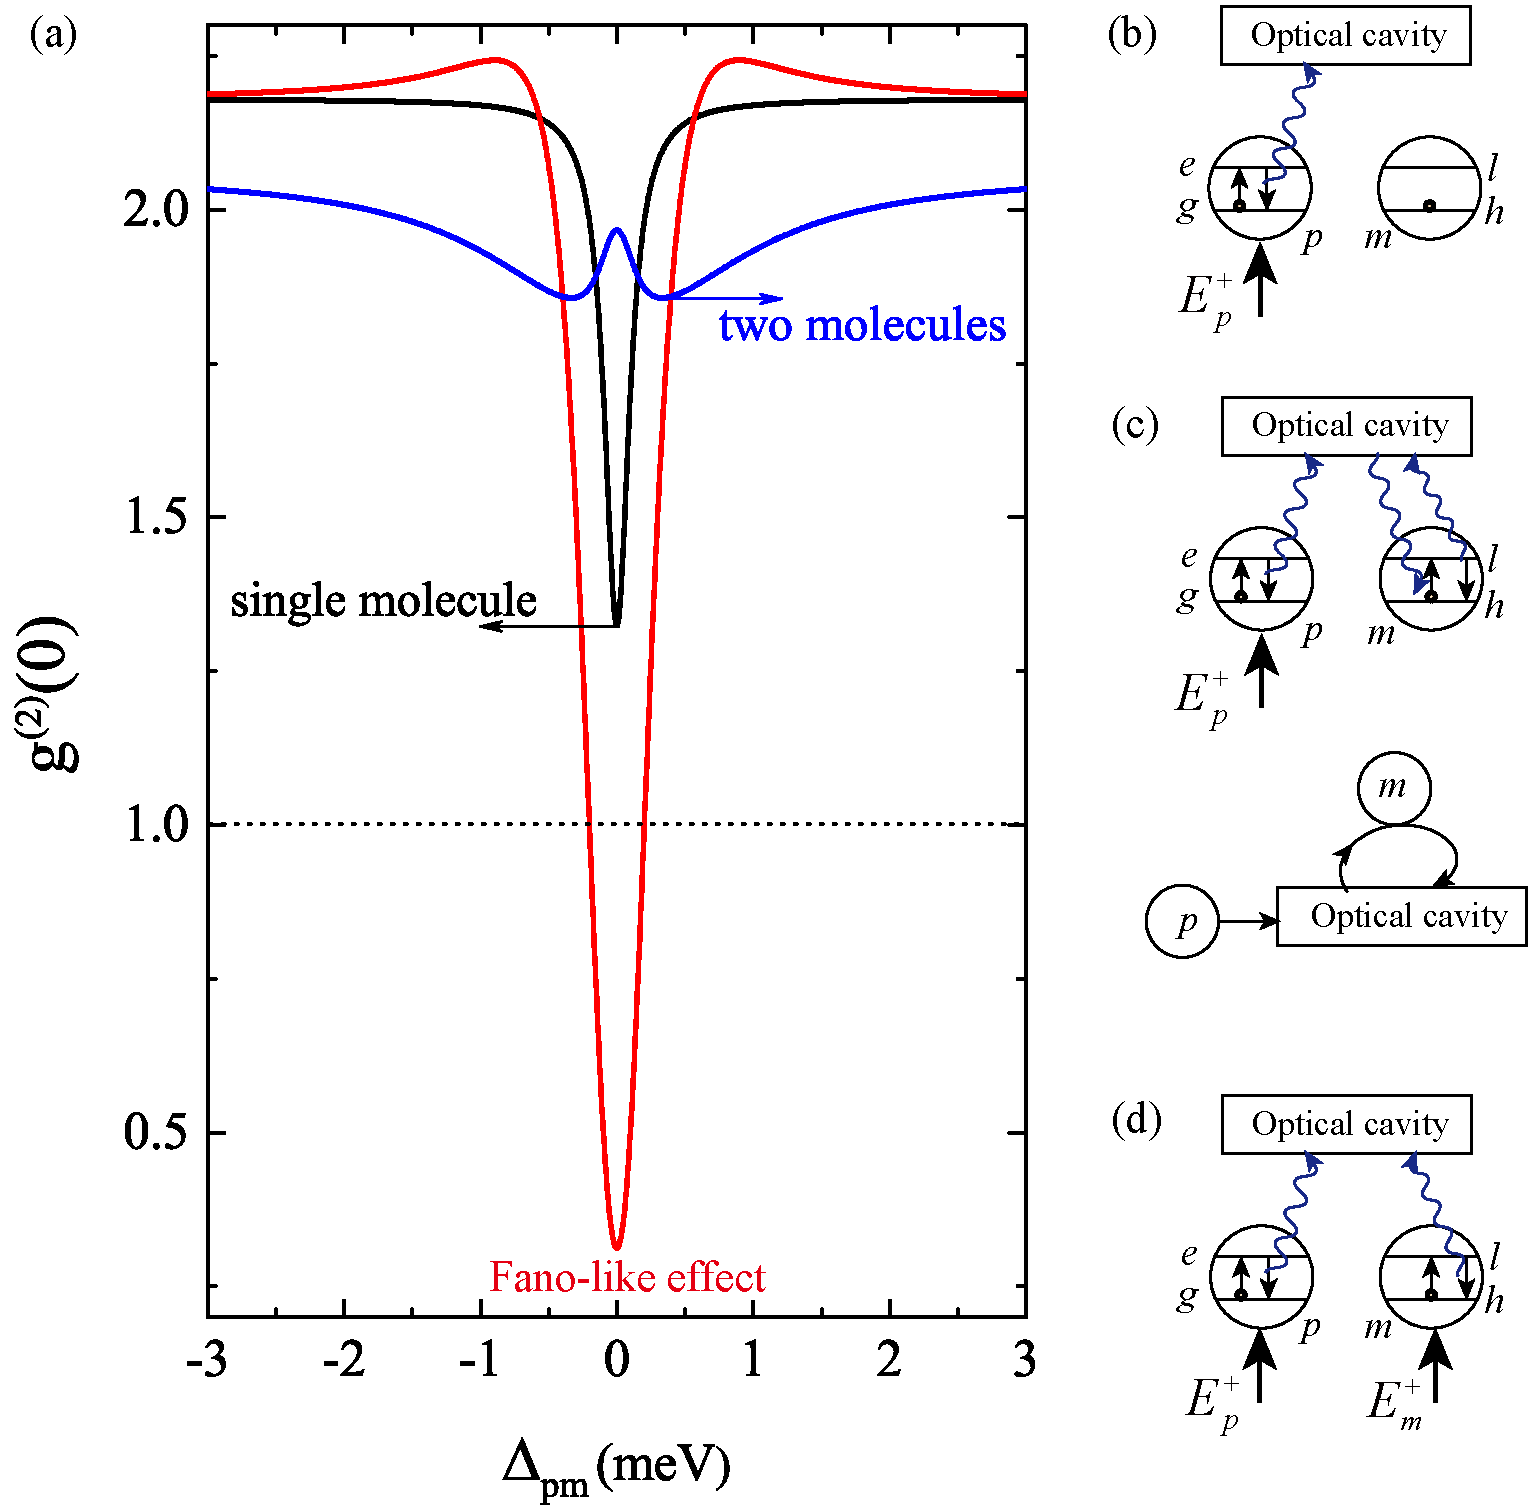
\includegraphics[width=0.45\textwidth]{fano-compare.pdf}
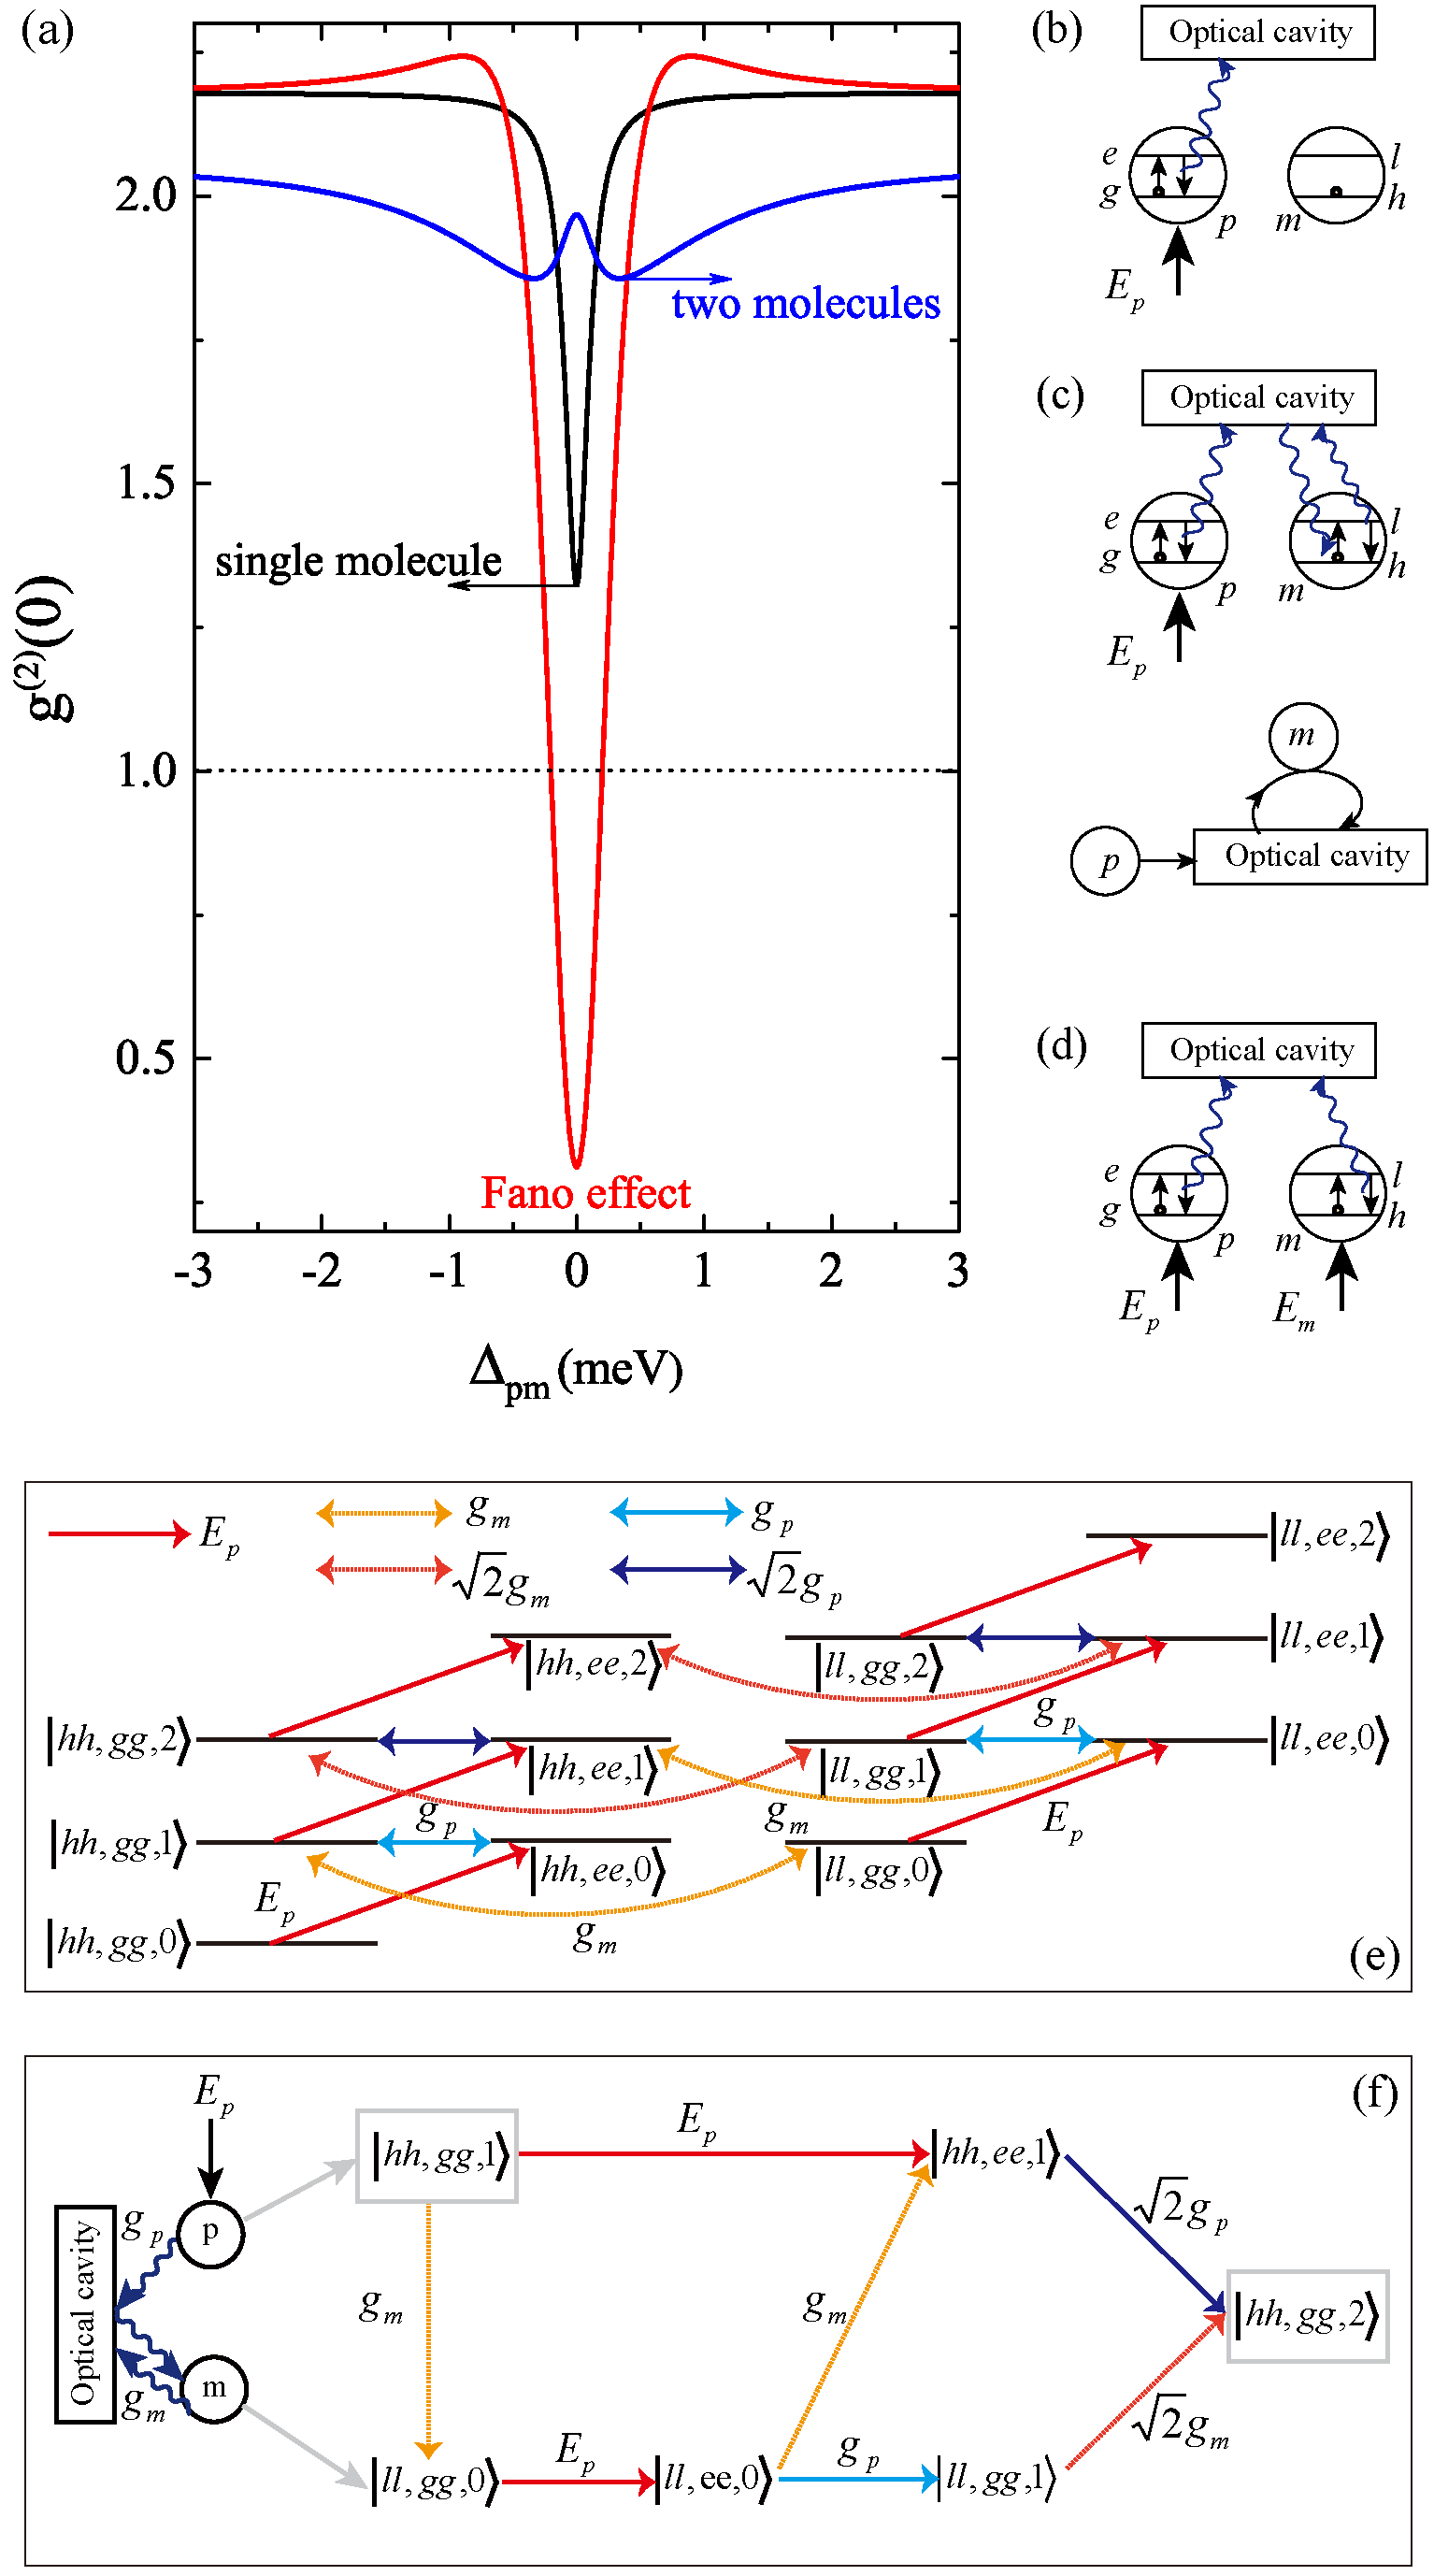
\includegraphics[width=0.4\textwidth]{fano-compare-mix.pdf}
\caption{(a) Second-order photon correlation function $g^{(2)}(0)$ as a function of the energy detuning between molecules and the cavity, where the detuning is defined as $\Delta_{pm}=\varepsilon_{e}-\varepsilon_{g}~(\varepsilon_{l}-\varepsilon_{h})$.
The corresponding mechanisms for single-molecule emission (b), emission due to Fano-like interference (c), and two-molecule emission (d) are displayed. 
(e) Excitation paths for two molecules $p$ and $m$ in a cavity, where the molecule $p$ is excited by an electrical pumping $E_{p}$ and its interaction with cavity is characterized by parameter $g_{p}$, while the molecule $m$ can only be excited by the cavity via electron-photon coupling $g_{m}$. (f) Two distinguishable transition pathways of two-photon excitations extracted from (e). The details for these matrix elements are provided in Section II of Ref.~\cite{SupplementalMaterial}. In our calculations,
we take $E_{p}=0.1~{\rm meV}$, $E_{m}=0.1~{\rm meV}$, $\gamma_{dp}=0.05~{\rm meV}$, $\gamma_{dm}=0.5~{\rm meV}$, $g_{p}=0.02~{\rm meV}$, $g_{m}=0.2~{\rm meV}$, $\gamma_{c}=0.02~{\rm meV}$, $\varepsilon_{l}=0.5~{\rm eV}$, $\varepsilon_{h}=-0.5~{\rm eV}$, $\varepsilon_{e}=0.5~{\rm eV}$, $\varepsilon_{g}=-0.5~{\rm eV}$, and $\hbar\omega_{c}=1.0~{\rm eV}$.
The above parameters are used throughout the paper, unless stated otherwise.}
\label{fano-compare}
\end{figure}

\subsection{Fano-like-effect-induced photon anti-bunching}
 First, we consider the single-molecule emission.
As shown in Fig.~\ref{fano-compare}(a), photon bunching can be observed in both on-resonance and off-resonance regions. 
%Note that, photon anti-bunching can also be observed for certain parameters in this case. This will be discussed in details in Fig.~\ref{fano-rp}.
Once the coupling between the second molecule $m$ and the cavity is turned on, $g_{m}\neq0$ and $E_{m}=0$, a strong photon anti-bunching appears in the resonant case.
Note that the molecule $m$ is not excited by the electrical pumping ($E_{m}=0$). Therefore, the antibuching behavior is a direct consequence of Fano-like interference effect.
To further clarify this, we present the corresponding fluorescence path in Fig.~\ref{fano-compare}(c). The electron in molecule $p$ can be excited by the pumping from level $g$ to $e$, it can relax to level $g$ by emitting a cavity photon. Thus, the optical cavity can be excited. The cavity can further excite the molecule $m$ near it by emitting a photon, resulting in creation of the molecular exciton.
The annihilation of the exciton emits the photon back to the cavity. One can see that the molecule $m$ can be regarded as a scatter for the excitation of the cavity. This is an evidence of the typical Fano interference effect \cite{PhysRev.124.1866,RevModPhys.82.2257}.


Hence, the Fano-like effect allows to achieve photon anti-bunching under electrical pumping. In detail, the Fano-like interference between the excitation of the cavity and the additional excitation from the molecule can suppress the emission of photon pairs while enhancing single-photon emission. To clarify this, we provide the corresponding excitation paths in Fig.~\ref{fano-compare}(e), in which we can extract two transition paths for two-photon excitations, as shown in Fig.~\ref{fano-compare}(f). Taking the coupled states as the basis, the first path is caused by the excitation of the molecule $p$, corresponding to $|hh,gg,1\rangle$ $\stackrel{E_{p}}{\longrightarrow}$ $|hh,ee,1\rangle$ $\stackrel{\sqrt{2}g_{p}}{\longrightarrow}$ $|hh,gg,2\rangle$. The second path only appears when the molecule $m$ without pumping is introduced, which can be  represented by $|hh,gg,1\rangle$ $\stackrel{g_{m}}{\longrightarrow}$ $|ll,gg,0\rangle$ $\stackrel{E_{p}}{\longrightarrow}$ $|ll,ee,0\rangle$ $\stackrel{g_{p}}{\longrightarrow}$ $|ll,gg,1\rangle$ $\stackrel{\sqrt{2}g_{m}}{\longrightarrow}$ $|hh,gg,2\rangle$.
Meanwhile, the molecule $m$ leads to a sub-path for the first one, that is, $|ll,ee,0\rangle$ $\stackrel{g_{m}}{\longrightarrow}$ $|hh,ee,1\rangle$.
As a consequence, we claim that the photon anti-bunching is caused by the quantum destructive interference between these two pathways. Notably, if the molecule $m$ is also excited by an electrical pumping $E_{m}$, more excitation paths are introduced, then the destructive interference is destroyed. As can be seen, the photon emitted from two-molecule emission case is bunched [Fig.~\ref{fano-compare}(a)]. Moreover, $g_{m}$-dependent photon statistics can also clarify the above discussions, see Section III of Ref.~\cite{SupplementalMaterial} for details.

%\begin{figure}[h]
%\centering
%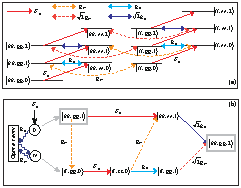
\includegraphics[width=0.48\textwidth]{mechanism-04.pdf}
%\caption{(a) Excitation paths for two molecules $p$ and $m$ in a cavity, where the molecule $p$ is excited by an electrical pumping $E_{p}$ and its interaction with cavity is characterized by parameter $g_{p}$, while the molecule $m$ can only be excited by the cavity via electron-photon coupling $g_{m}$. (b) Two distinguishable transition pathways of two-photon excitations extracted from (a). The details for these matrix elements are provided in Section I of the Supplemental Material \cite{SupplementalMaterial}}
%\label{fano-mechanism}
%\end{figure}

\subsection{Effect of quantity factor}
We now discuss how the photon anti-bunching is affected by the quantity factor $Q~(=\hbar\omega_{c}/\gamma_{c})$ of the cavity.
For low $Q$ ($g_{p},g_{m}\ll \gamma_{c}$, corresponding to bad-cavity limit) and small pumping $E_{p}$, the coupled single molecule and cavity system shows a near perfect single-photon emission [black line in Fig.~\ref{fano-rp}(a)].
This is because the cavity lifetime ($\propto 1/\gamma_{c}$) is short for low $Q$, such that no significant photon population can be stored in the cavity.
In this case, the emission of the molecule is close to the state without cavity, resulting in $g^{(2)}(0)\approx0$, similar to previous studies \cite{PhysRevB.70.115304,PhysRevA.91.061804,zhang2017electrically,PhysRevLett.122.233901}.
Compared with single- or two-molecule emission, the Fano-like effect can modify single-photon emission statistics while maintaining
a desired level of anti-bunching as shown from the blue and red lines in Fig.~\ref{fano-rp}(a).
For high $Q$ ($g_{p},g_{m}\gg \gamma_{c}$, corresponding to good-cavity limit), the photon can be stored effectively in the cavity. Thus, the condition of lasing is easily achieved in the case of single-molecule emission, leading to $g^{(2)}(0)\approx 1$ [black line in Fig.~\ref{fano-rp}(a)] and the photon statistics obey Poisson distribution [Fig.~\ref{fano-rp}(b)].
Interestingly, the crossover of the photon state from coherent and bunching to anti-bunching can be observed [Fig.~\ref{fano-rp}(b)].
This result clearly shows that the Fano-like effect redistributes the occupation probability of the cavity mode [Fig.~\ref{fano-rp}(b)-(d)].
 In Ref.~\cite{PhysRevLett.108.183601}, it is shown that an interference between the coherent light transmitted through the resonant cavity and the super-Poissonian light can lead to a strong photon anti-bunching in two cavities coupled to a quantum dot, while the effect vanishes in the absence of the cavity loss. Here, our results for high $Q$ are immune to this shortcoming.
 
 \begin{figure}[h]
\centering
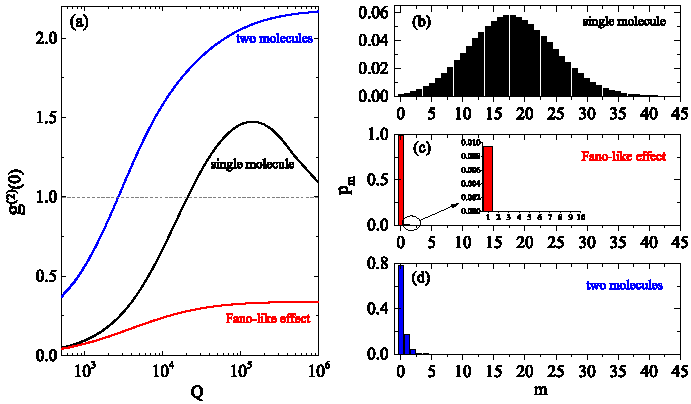
\includegraphics[width=0.48\textwidth]{fano-rp.pdf}
\caption{Left panel: (a) Second-order photon correlation function $g^{(2)}(0)$ as a function of the quantity factor $Q$ for three different cases shown in Fig.~\ref{fano-compare}. Right panel: The occupation probability of the cavity mode $p_{m}$ corresponding to Fig.~\ref{fano-rp} at $Q=10^{6}$.
For single-molecule emission, the photon statistics obey Poisson distribution (b), while introducing the Fano-like effect allows to obtain sub-Poisson distribution (c). The inset in (c) is an enlarged plot near $m=1$, where $p_{0}$ is not shown due to $p_{0}\gg p_{1}$. Photons  from the two-molecule emission follow super-Poisson distribution (d).}
\label{fano-rp}
\end{figure}

\begin{figure}[h]
\centering
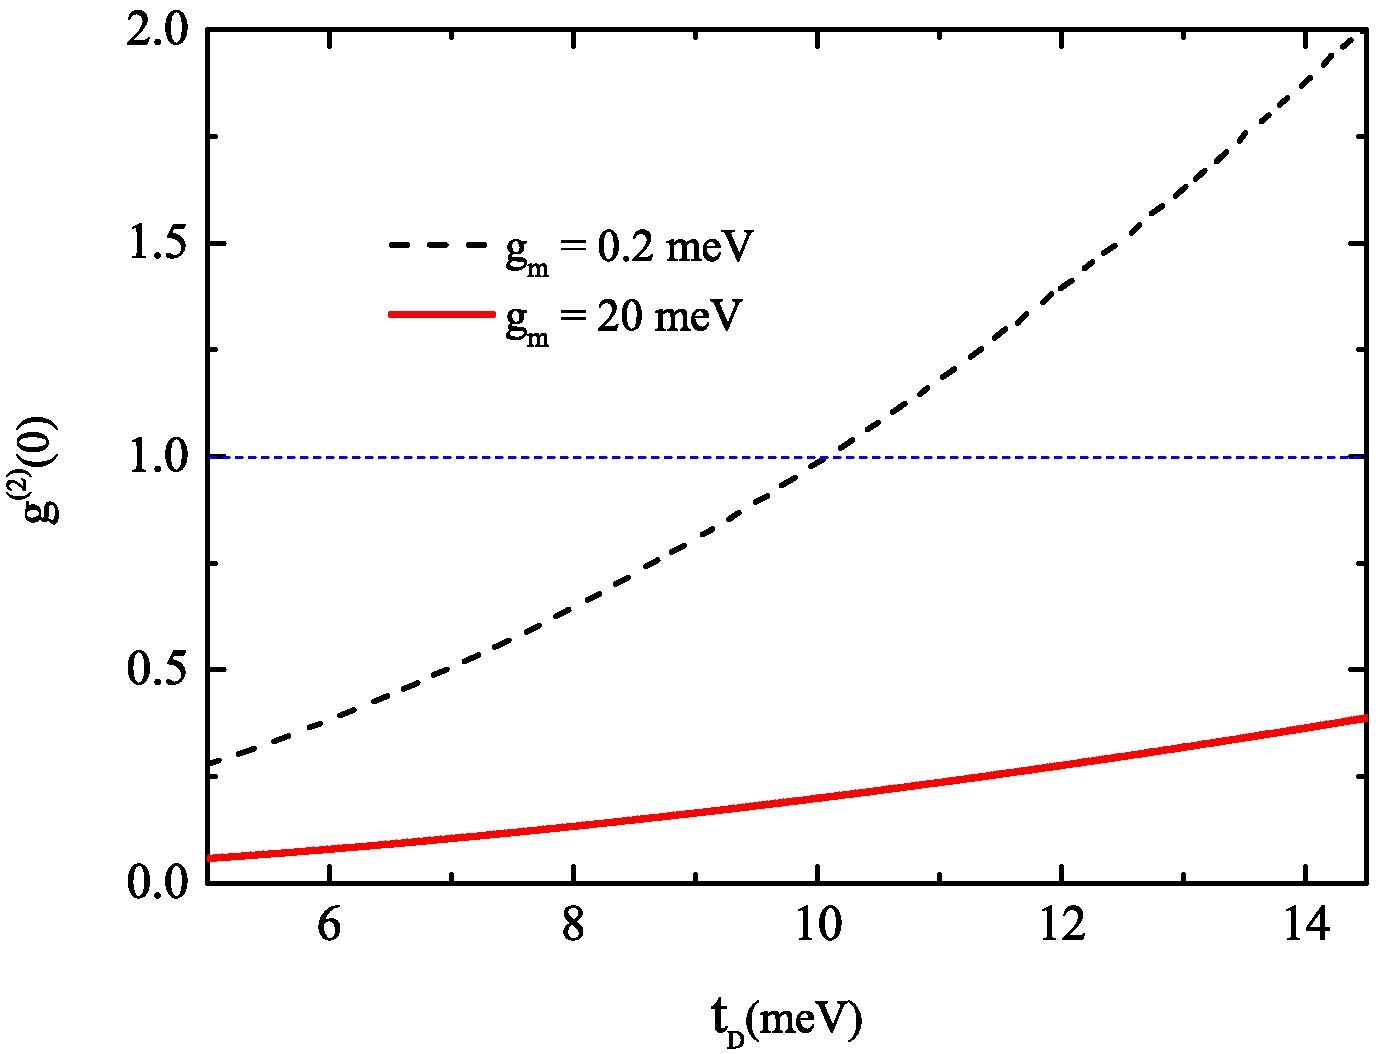
\includegraphics[width=0.4\textwidth]{fano-td.pdf}
\caption{Second-order photon correlation function $g^{(2)}(0)$ as a function of the dipole-dipole interaction $t_{D}$ for a cavity quality factor $Q=50$.}
\label{fano-td}
\end{figure}


 \subsection{Effect of dipole-dipole interaction}
 Above, our calculations ignore the dipole-dipole interaction between molecules. It only applies to the case when the inter-molecule distance is much larger than the characteristic length of dipole interaction. This requires a large cavity size. However, the dipolar interaction is unavoidable in situations like STM-induced electroluminescence \cite{zhang2016visualizing,PhysRevLett.122.233901}. Taking the parameters from such experiments, we can simulate the photon statistics of the emission with Fano-like interference in presence of the dipole-dipole interaction [Fig.~\ref{fano-td}]. Now, molecule $m$ can also be excited by molecule $p$ via the dipole-dipole interaction, represented by the parameter $t_{D}$. For $g_{m}\ll t_{D}$, the excitation of molecule $m$ by molecule $p$ dominates the photon emission process, such that $g^{(2)}(0)$ increases with $t_{D}$, and the transition from photon anti-bunching to bunching can be observed. Note that, for $g_{m}=0$, our results are consistent with a recent experiment \cite{PhysRevLett.122.233901}, where $g^{(2)}(0)$ for one molecule is smaller than the case of two molecules coupled through dipole interaction. For $g_{m}\gg t_{D}$, the photon emission with the Fano-like interference leads to a significant modification of the photon statistical properties. This provides an effective way to achieve the strong photon anti-bunching, and the reason has been explained in Fig.~\ref{fano-compare}(e)-(f). Remarkably, we find that the photon statistcs can be tuned from $g^{(2)}(0)=2$ to $g^{(2)}(0)=0.39$.


\section{Conclusions}
\revision{In summary, we provide unambiguous theoretical evidence for the role of the Fano-like interference effect on photon statistics in coupled molecule-cavity systems driven by electrical pumping. Control of photon statistics thus becomes possible by selectively electrical driving, even in the presence of the direct dipolar coupling between molecules. This way of achieving on-demand single photon emission using quantum interference can be realized in electrically biased STM-molecule junctions.}


%In summary, we have studied the photon statistics of molecules-cavity system that consists of two molecules and an optical cavity.
%By applying an electrical pumping to one of the molecules, photon bunching can be achieved. Once a second molecule without pumping is introduced to couple with the cavity, strong photon anti-bunching induced by the Fano-like interference effect appears. However, once electrical pumping to the second molecule is turned on, photon bunching is recovered. We have also studied the effect of direct dipolar coupling between molecules on the emitted photon statistics.
%Our results may be tested in the experiments where photon emission from molecular junction is driven by electrically biased STM tip.

%We note that the two molecules in our model can be placed near a STM tip \cite{PhysRevLett.109.186601,jiang2015distinguishing,zhang2016visualizing,PhysRevLett.122.233901,wu2019controllable,PhysRevLett.122.177401,dong2020microscopic} or a metal nanoparticle \cite{PhysRevB.76.125308,PhysRevB.77.165301,PhysRevLett.105.263601,PhysRevB.87.245313,PhysRevLett.108.233001}. For example, in the experiments of STM-induced molecular luminescence, the two molecules adsorbed on a metal substrate can be positioned nearby a STM tip. The electrons injected from the tip can excite one of the molecules locally ($p$ in our case), and the local plasmon mode in tip-substrate gap can also be excited either by the excited molecule or by the inelastic tunneling electrons directly. Consequently, the molecule $m$ nearby the tip can be excited by the excited plasmon mode.

\begin{acknowledgments}
This work is financially supported by the National Key Research and Development Program of China (Grant No. 2017YFA0403501), the National Natural Science Foundation of China (Grant No. 21873033), and the program for HUST academic frontier youth team. L.-L.N. acknowledges support from the China Postdoctoral Science Foundation (Grant No. 2020M672322).
\end{acknowledgments}

%

\bibliography{photon}
\end{document}

%
% ****** End of file apstemplate.tex ******

